% !TeX program = xelatex
% Arabic Dyslexia-Friendly Text Simplification Assistant
% Execution Plan: milestones, difficulties, and mitigations
\documentclass[11pt,a4paper]{article}

% ---------- Layout ----------
\usepackage[margin=2.2cm]{geometry}
\usepackage{fontspec}

% ---------- Graphics / diagrams ----------
\usepackage{tikz}
\usetikzlibrary{arrows.meta,shapes.geometric,positioning,fit,backgrounds,calc,decorations.pathreplacing,shadows}
\usepackage{graphicx}
\usepackage{caption}

% ---------- Tables / lists / boxes ----------
\usepackage{booktabs}
\usepackage{array}
\usepackage{longtable}
\usepackage{enumitem}
\usepackage{tcolorbox}
\tcbuselibrary{skins,breakable}
\usepackage{xcolor}

% ---------- References / misc ----------
\usepackage{hyperref}
\usepackage{microtype}
\usepackage{parskip}

% ---------- Colors (matching pipeline_architecture.tex) ----------
\definecolor{stagecolor}{RGB}{255,229,204}
\definecolor{iocolor}{RGB}{214,240,214}
\definecolor{blockcolor}{RGB}{214,228,246}
\definecolor{cloudcolor}{RGB}{240,224,247}
\definecolor{devicecolor}{RGB}{214,242,240}
\definecolor{prosgreen}{RGB}{39,116,66}
\definecolor{consred}{RGB}{160,39,39}
\definecolor{prosbg}{RGB}{234,247,238}
\definecolor{consbg}{RGB}{252,235,235}
\definecolor{headnavy}{RGB}{22,45,74}
\definecolor{amberbg}{RGB}{255,244,224}
\definecolor{amber}{RGB}{184,120,10}

\hypersetup{
  colorlinks=true,
  linkcolor=headnavy,
  citecolor=headnavy,
  urlcolor=headnavy,
  pdftitle={Execution Plan: Milestones, Difficulties, and Mitigations},
  pdfauthor={Samsung Innovation Campus Capstone Candidate}
}

% ---------- TikZ styles reused from pipeline_architecture.tex ----------
\tikzset{
  block/.style={rectangle, draw=black!70, thick, rounded corners, fill=blockcolor,
    minimum width=2.6cm, minimum height=1.05cm, align=center, font=\small, drop shadow},
  stage/.style={rectangle, draw=black!70, thick, rounded corners, fill=stagecolor,
    minimum width=2.8cm, minimum height=1.2cm, align=center, font=\small\bfseries, drop shadow},
  iodata/.style={rectangle, draw=black!60, thick, rounded corners, fill=iocolor,
    minimum width=2.5cm, minimum height=1cm, align=center, font=\small, drop shadow},
  lbl/.style={font=\scriptsize\itshape, text=black!60, fill=white, inner sep=1pt},
  myarrow/.style={-{Latex[length=2.8mm,width=2mm]}, thick},
  dimarrow/.style={-{Latex[length=2.4mm,width=1.6mm]}, thick, dashed, black!55},
}

% ---------- Box environments ----------
\newtcolorbox{noteb}[1][]{
  colback=blue!4, colframe=headnavy, boxrule=0.5pt, arc=2pt,
  left=6pt, right=6pt, top=4pt, bottom=4pt, #1
}
\newtcolorbox{goalbox}[1][]{
  colback=prosbg, colframe=prosgreen, boxrule=0.6pt, arc=2pt,
  title=\textbf{Goal / Exit Criterion}, fonttitle=\bfseries, coltitle=white,
  colbacktitle=prosgreen, top=2pt, bottom=2pt, left=4pt, right=4pt, #1
}
\newtcolorbox{milestonehead}[2]{
  colback=headnavy!6, colframe=headnavy, boxrule=0.7pt, arc=2pt, breakable,
  title={\textbf{#1}\hfill\normalfont\footnotesize\textcolor{white}{#2}},
  fonttitle=\bfseries\large, coltitle=white, colbacktitle=headnavy,
  top=3pt, bottom=3pt, left=5pt, right=5pt
}

\title{\vspace{-1.5cm}\textbf{\Large Execution Plan}\\[4pt]
\large Milestones, Difficulties, and Mitigations \\[2pt]
\normalsize\itshape Arabic Dyslexia-Friendly Text Simplification Assistant}
\author{Samsung Innovation Campus --- Capstone Candidate Idea Brief}
\date{September 2026}

\begin{document}
\maketitle
\vspace{-0.8cm}

\begin{noteb}
\textbf{Purpose of this document.} This is a companion to
\emph{Pipeline Architecture, Data Flow, and Feasibility Analysis}. That
document settles \emph{what} we are building and \emph{why}; this document
breaks the 20-day schedule (the Execution Timeline Gantt chart in the
pipeline report) into concrete, checkable milestones, and for each one lists what is
likely to go wrong and how the team plans to respond --- so problems have an
agreed response \emph{before} they happen, not during a scramble.
\end{noteb}

\tableofcontents
\thispagestyle{empty}
\newpage

% =====================================================================
\section{How to Read This Document}
% =====================================================================

The plan is organized into six groups (A--F), matching the six task groups
in the pipeline report's Gantt chart. Each group contains one or more
milestones. Every milestone has the same four parts:

\begin{itemize}[leftmargin=1.4em]
  \item \textbf{Goal / exit criterion} --- a concrete, checkable definition
  of ``done,'' not a vague activity description. If the exit criterion can't
  be checked in five minutes, it isn't specific enough.
  \item \textbf{Key steps} --- the short sequence of actions to get there.
  \item \textbf{Difficulties \& mitigations} --- what is likely to go wrong,
  paired one-to-one with the team's planned response. These are not
  hypothetical; several are pulled directly from the risk register in the
  pipeline report (marked \textbf{[R\#]} where applicable).
  \item \textbf{Suggested owner role} --- a role, not a name, so the team can
  assign specific people at kickoff without this document going stale.
\end{itemize}

\begin{noteb}
\textbf{A rule for using this document during the sprint.} If a milestone's
exit criterion is not met by the end of its window, that is the trigger to
apply the mitigation immediately, not a reason to quietly extend the
deadline. Section~\ref{sec:critical-path} lists which milestones are allowed
to slip without threatening the overall timeline, and which are not.
\end{noteb}

% =====================================================================
\section{Milestone Overview}
% =====================================================================

\begin{center}
\small
\begin{longtable}{@{}p{0.7cm}p{4.4cm}p{1.6cm}p{5.3cm}p{2.6cm}@{}}
\toprule
\textbf{ID} & \textbf{Milestone} & \textbf{Days} & \textbf{Exit Criterion} & \textbf{Owner role} \\
\midrule
\endhead
\multicolumn{5}{@{}l}{\textit{Group A --- Validation \& Setup (Week 0)}} \\
A1 & Fast pilot: BAREC$\to$Gemini generation & 1--2 & A sample of $\sim$50 filtered pairs exists with a measured yield rate & NLP lead \\
A2 & Validation-partner outreach & 1--5 & A named contact confirmed, or fallback formally activated & PM / outreach lead \\
A3 & Hand-label DSPy validation set & 2--5 & 30--100 labeled triples, with a pre-agreed target agreement metric & Whole team (split) \\
\addlinespace
\multicolumn{5}{@{}l}{\textit{Group B --- Stage 1: Simplify (Week 1--2)}} \\
B1 & Judge pilot \& selection & 4--8 & One judge model chosen against the hand-labeled set, bias-checked & NLP lead \\
B2 & Synthetic data generation at scale & 4--7 & Filtered training set at or above the yield target from A1 & NLP lead \\
B3 & AraT5 fine-tuning & 7--12 & A checkpoint that beats the un-tuned baseline on held-out eval & ML engineer \\
\addlinespace
\multicolumn{5}{@{}l}{\textit{Group C --- Stage 2: Diacritize (Week 2)}} \\
C1 & Diacritizer integration \& domain validation & 9--13 & CATT (or fallback) validated on Stage~1's own output, not just Tashkeela & ML engineer \\
\addlinespace
\multicolumn{5}{@{}l}{\textit{Group D --- Stage 3: Read Aloud (Optional, Week 1--2)}} \\
D1 & TTS engine decision \& integration & 6--10 & A working TTS call with either native or aligned word timing --- or a documented cut decision & TTS / frontend eng. \\
D2 & Word-sync highlight UI \& display-diacritics decision & 10--15 & Karaoke-style highlighting works on a recorded sample; on-screen diacritic density decided, not assumed & Frontend eng. \\
\addlinespace
\multicolumn{5}{@{}l}{\textit{Group E --- Integration \& Polish (Week 2--3)}} \\
E1 & End-to-end pipeline wiring & 13--16 & A single typed sentence flows through every enabled stage without manual intervention & Integration lead \\
E2 & Runtime faithfulness gate (stretch) & 16--18 & Live low-score outputs fall back to original text with a note & NLP lead \\
E3 & Testing \& bug-fix buffer & 16--19 & No open blocker bugs; at least one real read-through by a human tester if available & Whole team \\
\addlinespace
\multicolumn{5}{@{}l}{\textit{Group F --- Submission}} \\
F1 & Pitch \& submission prep & 20 & Deck + demo ready; on-device/cloud framing stated honestly & PM / whole team \\
\bottomrule
\end{longtable}
\end{center}

\newpage
% =====================================================================
\section{Dependency Flow}
\label{sec:critical-path}
% =====================================================================

\begin{figure}[h!]
\centering
\resizebox{\textwidth}{!}{%
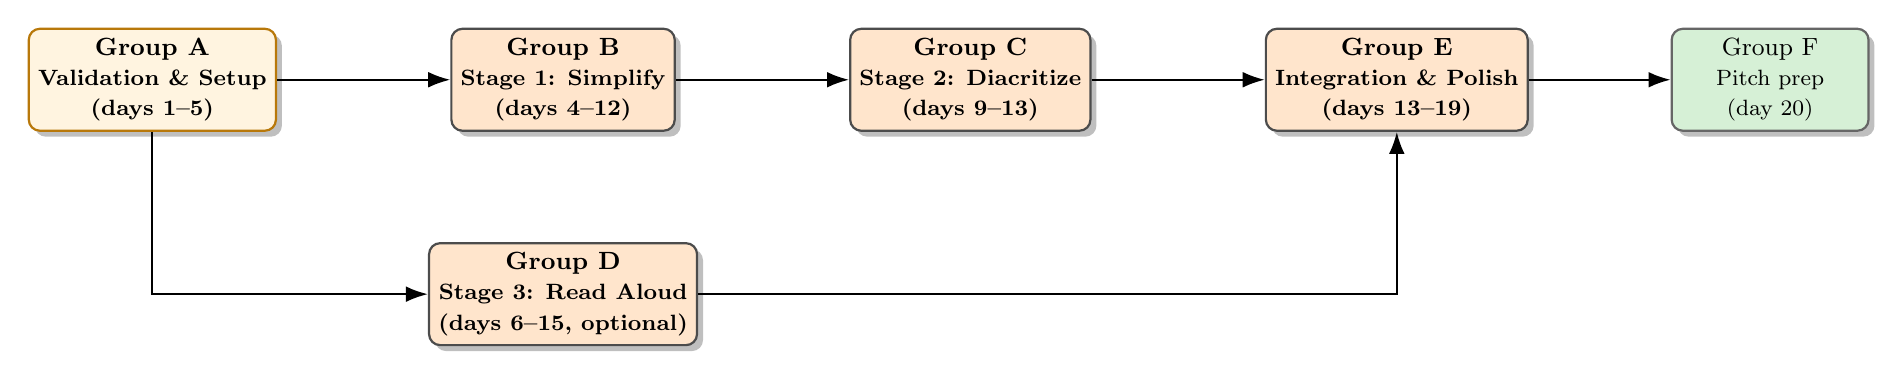
\begin{tikzpicture}[node distance=8mm and 10mm]

\node[stage, fill=amberbg, draw=amber] (A) {Group A\\\footnotesize Validation \& Setup\\\footnotesize (days 1--5)};
\node[stage, right=22mm of A] (B) {Group B\\\footnotesize Stage 1: Simplify\\\footnotesize (days 4--12)};
\node[stage, right=22mm of B] (C) {Group C\\\footnotesize Stage 2: Diacritize\\\footnotesize (days 9--13)};
\node[stage, below=14mm of B] (D) {Group D\\\footnotesize Stage 3: Read Aloud\\\footnotesize (days 6--15, optional)};
\node[stage, right=22mm of C] (E) {Group E\\\footnotesize Integration \& Polish\\\footnotesize (days 13--19)};
\node[iodata, right=18mm of E] (F) {Group F\\\footnotesize Pitch prep\\\footnotesize (day 20)};

\draw[myarrow] (A) -- (B);
\draw[myarrow] (B) -- (C);
\draw[myarrow] (A) |- (D);
\draw[myarrow] (C) -- (E);
\draw[myarrow] (D) -| (E);
\draw[myarrow] (E) -- (F);

\end{tikzpicture}}
\caption{Milestone-group dependencies. Groups B and D both start from Group
A's outputs and run in parallel --- Group D (optional) can be cut entirely
without blocking Group C or E. Group E cannot start in earnest until both
Group C and (if kept) Group D have produced something to integrate.}
\label{fig:dependency-flow}
\end{figure}

\begin{noteb}
\textbf{Which milestones can slip, and which cannot.} A2 (partner outreach)
and B1 (judge selection) are the two milestones on the true critical path:
A2 gates the credibility of the whole pitch (Section~\ref{sec:top-risks}),
and B1 gates B2 and B3, which gate everything in Groups C and E. D1/D2
(Stage~3) are explicitly allowed to slip or be cut per
Section~\ref{sec:group-d} without threatening submission. E2 (runtime gate)
is a stretch goal by design and is the first thing dropped if E1 or E3 run
long.
\end{noteb}

\newpage
% =====================================================================
\section{Group A --- Validation \& Setup (Days 1--5)}
% =====================================================================

\begin{milestonehead}{A1 --- Fast Pilot: BAREC $\to$ Gemini Generation}{Days 1--2}
\begin{goalbox}
A small sample ($\sim$50--100 BAREC sentences) has been run through Gemini
generation and the DSPy-style dual filter (equivalence + readability drop),
producing a measured yield rate (\% of pairs that survive) to calibrate
Group B's targets before committing full-scale effort.
\end{goalbox}

\textbf{Key steps:} pick 2--3 BAREC genres and a mid-to-high readability
band to sample from; write and test the generation prompt; hand-check a
subset of outputs for obvious quality problems before trusting the
automatic filter's numbers.

\begin{center}
\small
\begin{tabular}{@{}p{6.3cm}p{6.9cm}@{}}
\toprule
\textbf{Difficulty} & \textbf{Mitigation} \\
\midrule
API access/quota not yet set up, burning day~1 on logistics instead of
signal. & Verify API keys and a minimal working call \emph{before} day~1
begins, as a pre-sprint checklist item, not part of this milestone's clock. \\
\addlinespace
Genre/level chosen for the pilot turns out unrepresentative (e.g.\ picking
an easy genre inflates the apparent yield). & Sample across at least two
genres and two readability bands in the very first pilot batch, not one, so
the yield number reflects a range rather than a lucky draw. \\
\addlinespace
No DSPy judge exists yet at this point, so filtering can't be automated the
way B1 will do it. & For this pilot only, filter by quick manual read
(2--3 team members skim the batch) to get a directional yield estimate; this
is deliberately informal and gets replaced by the real judge in B1. \\
\bottomrule
\end{tabular}
\end{center}
\end{milestonehead}

\vspace{6pt}
\begin{milestonehead}{A2 --- Validation-Partner Outreach}{Days 1--5}
\begin{goalbox}
By end of day~5, either a named contact (school, org, or individual dyslexic
Arabic reader) has agreed to give feedback during the sprint, \textbf{or} the
informal-tester fallback has been formally activated and written into the
pitch narrative. This milestone does not end in an ambiguous ``still
waiting'' state.
\end{goalbox}

\textbf{Key steps:} build a target list on day~1 (schools, learning-disability
orgs, the previously identified individual lead, authors of the cited prior
work on Arabic dyslexic-text correction and dyslexia-friendly typeface
design); reach out through multiple channels in parallel, not sequentially;
set the day-5 decision checkpoint on the calendar in advance.

\begin{center}
\small
\begin{tabular}{@{}p{6.3cm}p{6.9cm}@{}}
\toprule
\textbf{Difficulty} & \textbf{Mitigation} \\
\midrule
\textbf{[R1]} No partner responds within the window --- the single highest
likelihood/impact risk in the pipeline report. & Use multiple parallel
channels from day~1 (email, personal networks, direct messages, school
visits) rather than one cold-email pass and a wait; treat non-response by
day~3 as a signal to add more targets, not to wait longer on the same ones. \\
\addlinespace
Outreach reaches people, but too late in the week to get usable feedback
before Group~E's testing buffer. & Prioritize the already-identified
individual lead and the cited papers' authors first, since they are the
fastest-to-respond channels, before broader cold outreach to institutions. \\
\addlinespace
A contact agrees in principle but can't commit to concrete time during the
sprint. & Ask explicitly for the smallest useful commitment up front (a
single 15-minute read-aloud session in Group~E), not open-ended
availability, so ``yes'' actually converts to usable feedback later. \\
\addlinespace
No human-outcome evidence exists anywhere in the plan beyond the automatic
equivalence/readability score. & If any partner is secured, reserve one
concrete slot in E3 for a real before/after reading check (speed or
self-reported ease) --- even one data point beats zero for the pitch. \\
\bottomrule
\end{tabular}
\end{center}
\end{milestonehead}

\newpage
\begin{milestonehead}{A3 --- Hand-Label the DSPy Validation Set}{Days 2--5}
\begin{goalbox}
Real annotated (original, simplified, verdict) triples exist, covering
both positive and negative equivalence cases, with enough volume and class
balance to compile a validator against.
\end{goalbox}

\textbf{Status: done, and ongoing.} The original plan (manually write
positives, deliberately corrupt some for negatives) was superseded by a
better approach: a web review tool (``Pilot Pair Review,'' a Claude
Artifact with a shared realtime database) lets a reviewer annotate the
pilot's own \emph{real} generated pairs directly --- \texttt{level\_verdict}
and \texttt{equiv\_verdict} per pair, plus notes --- rather than writing
synthetic examples from scratch. Current volume: 102 usable equivalence
annotations (65 equivalent / 37 not-equivalent --- the not-equivalent count
includes ``ok'' confirmations of an already-negative original verdict, not
just explicit corrections) and 12 level corrections. This directly fed
\texttt{scripts/optimize\_equivalence\_validator.py}'s MIPROv2 compile
(Section on validator calibration in the pipeline report): raw 48.0\%
$\to$ compiled 66.7\% accuracy on held-out pairs. Level annotations remain
thinner (12, corrections-only, no confirmations yet) and are not yet
sufficient on their own to recalibrate the level classifier, which is
compiled against BAREC's own labels instead (see B1). Annotation continues
in the background; more level corrections specifically are the highest-value
next additions.

\begin{center}
\small
\begin{tabular}{@{}p{6.3cm}p{6.9cm}@{}}
\toprule
\textbf{Difficulty} & \textbf{Mitigation} \\
\midrule
With one reviewer doing the labeling, their judgment calls define
``correct'' for the whole downstream validator. & No second labeler has
been added yet; treat compiled accuracy numbers as reflecting one
reviewer's standard until cross-checked, and consider a second reviewer
for a sample if time allows. \\
\addlinespace
Real generated pairs are overwhelmingly positive (most simplifications
pass), so negative examples accumulate slowly. & The real negative count
(37) is higher than it first appears because ``ok'' confirmations of an
already-failing original verdict count too --- worth checking this before
assuming more explicit corrections are needed. \\
\bottomrule
\end{tabular}
\end{center}
\end{milestonehead}

\newpage
% =====================================================================
\section{Group B --- Stage 1: Simplify (Days 4--12)}
% =====================================================================

\begin{milestonehead}{B1 --- Generator + Validators Pilot (2\%)}{Days 4--8}
\begin{goalbox}
BAREC's 67,601 level-1--4 sentences (level~5 dropped) are loaded and split
three ways at sampling time: easy band (levels~1--2, identity pairs), hard
band (levels~3--4, generated and validated), and scripture-sourced
sentences (Quran/Hadith/Old/New Testament, identity pairs regardless of
level --- see the pipeline report's content-safety section). A stratified
2\% sample (1,350 sentences: 708 easy / 606 hard / 36 scripture) has run
through the DeepSeek generator and both DSPy validators, with a measured
pass rate.
\end{goalbox}

\textbf{Status: done.} Both validators are now optimizer-compiled against
real ground truth, not zero-shot: \texttt{ClassifyReadabilityLevel} via
\texttt{dspy.BootstrapFewShot} against 1,000 balanced BAREC-labeled
sentences (79.7\% easy/hard band accuracy, 53.0\% exact match, 7/800
failures on a held-out 800-sentence set --- a \texttt{dspy.MIPROv2}
alternative was tried and reverted after it introduced a 2--3$\times$
higher parse-failure rate for no real accuracy gain, see the pipeline
report); \texttt{CheckSemanticEquivalence} via \texttt{dspy.MIPROv2}
against 102 human-annotated pairs from A3 (66.7\% accuracy, up from 48.0\%
zero-shot). \texttt{scripts/barec\_simplification\_pipeline.py} loads both
compiled programs automatically. The scripture-preservation fix
(Quran/Hadith/Bible sentences routed to identity pairs) was added after an
earlier completed pilot run was found to have generated 28 scripture
rewrites before the fix existed --- caught by the reviewer, not by any
automated check, which is itself a lesson for what else might need an
explicit content-safety rule rather than relying on the validators alone.

\begin{center}
\small
\begin{tabular}{@{}p{6.3cm}p{6.9cm}@{}}
\toprule
\textbf{Difficulty} & \textbf{Mitigation} \\
\midrule
\textbf{[R2]} The generator and both validators all run on the same model
(DeepSeek) for this pilot --- a model can share blind spots with itself
across roles, so a generation error and the equivalence check meant to
catch it are not fully independent. & Not yet done: spot-check a sample of
pilot output with a second model before trusting the pass rate at face
value; still an open item for full-scale generation, not just a pilot
formality. \\
\addlinespace
2\% is a small pilot; the real pass rate at full hard-band scale (31,744
sentences) is unknown until B2 runs. & Treat the pilot's measured pass rate
as the number that decides whether B2 is worth running at full scale ---
still the plan, not yet executed. \\
\addlinespace
Content-safety issues (like the scripture case) can exist in categories the
validators were never designed to catch, since they check meaning
preservation and difficulty, not canonicity. & Treat this as a standing
question for full-scale generation: are there other source categories in
BAREC (e.g.\ legal/official text) that deserve the same kind of
identity-pair carve-out, not just scripture? Worth a deliberate review
before B2, not an assumption that scripture was the only case. \\
\bottomrule
\end{tabular}
\end{center}
\end{milestonehead}

\newpage
\begin{milestonehead}{B2 --- Generation at Full Hard-Band Scale}{Days 4--7}
\begin{goalbox}
Every hard-band anchor (up to 31,744 sentences, budget permitting) has been
run through the generator and both validators; the filtered hard pairs,
combined with the full easy-band identity set, form the training data
handed to B3.
\end{goalbox}

\textbf{Key steps:} scale B1's pipeline up from the 2\% pilot; batch
sentences per API call; track pass rate daily against B1's pilot baseline;
combine filtered hard pairs with the (separately filtered) easy-band
identity pairs into one training set.

\begin{center}
\small
\begin{tabular}{@{}p{6.3cm}p{6.9cm}@{}}
\toprule
\textbf{Difficulty} & \textbf{Mitigation} \\
\midrule
\textbf{[R3]} Pairs pass the equivalence check but the output doesn't
actually read as easy-band. & The dual validator design already requires
both checks independently, not a combined score --- if pass rate is low,
check which validator is rejecting more often to isolate whether the
problem is faithfulness or simplification strength. \\
\addlinespace
BAREC's religious/highly formal reference genres are a poor stylistic match
for conversational simplification and may silently drag down hard-band
pass rate. & Break down B1's pilot pass rate by \texttt{Domain}/\texttt{Source}
before scaling up; deprioritize or separately handle weak genres rather than
discovering this after a full-scale run. \\
\addlinespace
Pass rate at full scale turns out much lower than B1's pilot suggested. &
Monitor daily against the B1 baseline; if it drops significantly, revisit
the generator's instructions before loosening either validator's bar, since
faithfulness matters more than yield. \\
\addlinespace
Per-call instruction overhead inflates cost/time at 31,744-sentence scale. &
Batch many sentences per API call, per the pipeline report's cost analysis
--- though at DeepSeek's pricing this is a minor concern even unbatched. \\
\bottomrule
\end{tabular}
\end{center}
\end{milestonehead}

\newpage
\begin{milestonehead}{B3 --- AraT5 Fine-Tuning}{Days 7--12}
\begin{goalbox}
A fine-tuned AraT5 checkpoint exists that scores higher than the un-tuned
baseline on the B1 judge run over a held-out BAREC split, and the checkpoint
is small enough to quantize for on-device deployment.
\end{goalbox}

\textbf{Key steps:} fix hyperparameters up front (informed by AraT5-MSAizer's
published settings rather than a from-scratch search); checkpoint
frequently; run the held-out eval as soon as a checkpoint looks stable,
not only at the very end.

\begin{center}
\small
\begin{tabular}{@{}p{6.3cm}p{6.9cm}@{}}
\toprule
\textbf{Difficulty} & \textbf{Mitigation} \\
\midrule
\textbf{[R4]} Compute/time only allows one or two full fine-tuning cycles
within the sprint. & Fix hyperparameters from precedent (AraT5-MSAizer)
instead of searching; treat the first full run as the one that ships unless
it clearly fails the held-out eval, to avoid an open-ended tuning loop. \\
\addlinespace
Model quality is bounded by B2's synthetic-pair quality --- there is no
real ground-truth simplification anywhere in the pipeline, so fine-tuning
can only be as good as generation-plus-filtering allowed it to be. &
Treat B1/B2 as the true quality ceiling and invest debugging time there
first if B3's eval score disappoints, rather than assuming the fine-tuning
step itself is the problem. \\
\addlinespace
A mid-run failure (crash, bad hyperparameter, corrupted checkpoint) costs
an entire compute slot with only one or two cycles available. &
Checkpoint frequently and keep the previous stable checkpoint until the new
one is confirmed better on held-out eval, so a bad run never costs more
than the time since the last checkpoint. \\
\bottomrule
\end{tabular}
\end{center}
\end{milestonehead}

\vspace{6pt}
\begin{noteb}
\textbf{B1.5 --- Candidate reranking and a fine-tuned classifier (in
progress, not yet started).} A next-phase change to B1's design, informed
by the actual TSAR~2025 Shared Task on Readability-Controlled Text
Simplification: replace B1's binary pass/fail validator gate with
generate-N-candidates-then-rerank, scored by (a) a classifier fine-tuned
on the full BAREC corpus rather than the few-shot \texttt{ClassifyReadabilityLevel},
and (b) the equivalence validator. See the pipeline report's section on
this for the full rationale, including why a from-scratch autoencoder was
considered and rejected. Currently blocked on external GPU compute
(Colab/Kaggle) --- the development machine has no CUDA GPU. If time
allows, this replaces B2's simple gating before full-scale generation;
if not, B2 proceeds with the current binary-gate design and this becomes
a documented future-work item for the pitch rather than a shipped
improvement.
\end{noteb}

\newpage
% =====================================================================
\section{Group C --- Stage 2: Diacritize (Days 9--13)}
% =====================================================================

\begin{milestonehead}{C1 --- Diacritizer Integration \& Domain Validation}{Days 9--13}
\begin{goalbox}
CATT's encoder-decoder checkpoint (or the Fine-Tashkeel/ByT5 fallback) is
integrated, fine-tuned on Tashkeela plus a sample of B3's own simplified
output, and validated to preserve base letters on that domain --- not just
on Tashkeela's native classical/religious text.
\end{goalbox}

\textbf{Key steps:} run CATT out-of-the-box on a sample of Stage~1 output
first, to get a baseline before any domain fine-tuning; fine-tune on a
Tashkeela + Stage~1-sample mix; build an automated base-letter comparison
check (input letters vs.\ output letters, ignoring diacritic marks).

\begin{center}
\small
\begin{tabular}{@{}p{6.3cm}p{6.9cm}@{}}
\toprule
\textbf{Difficulty} & \textbf{Mitigation} \\
\midrule
\textbf{[R6]} A diacritizer trained on classical/religious Tashkeela text
underperforms on simplified, contemporary sentences. & Validate on a sample
of B3's actual output specifically, starting day~9, not only on Tashkeela's
native domain; fine-tune further on a blended sample if the baseline check
is weak. \\
\addlinespace
CATT's generative (encoder-decoder) checkpoint is empirically more accurate
but is not structurally prevented from altering base letters, unlike a
tagging model. & Build the base-letter-preservation check as an explicit
automated test before trusting output read aloud verbatim in Stage~3;
flag or reject any output where base letters changed. \\
\addlinespace
Diacritization errors are read aloud verbatim by Stage~3 --- an incorrect
mark becomes an audible wrong sound, more user-visible than in most
diacritization use cases. & Treat this stage's error rate as higher-stakes
than a typical diacritization benchmark would suggest; do not lower the
validation bar just because CATT reports strong aggregate numbers on a
different domain. \\
\bottomrule
\end{tabular}
\end{center}
\end{milestonehead}

\newpage
% =====================================================================
\section{Group D --- Stage 3: Read Aloud (Optional, Days 6--15)}
\label{sec:group-d}
% =====================================================================

\begin{noteb}
\textbf{This whole group is optional.} A text-only pipeline (typed input
$\to$ simplified $\to$ diacritized output) is already a complete, demoable
product without Stage~3. Both milestones below carry an explicit cut
decision, not just a mitigation, because forcing a compromised Stage~3
implementation is worse for the pitch than a clean two-stage product.
\end{noteb}

\begin{milestonehead}{D1 --- TTS Engine Decision \& Integration}{Days 6--10}
\begin{goalbox}
Either (a) a TTS engine is integrated with confirmed word-level timing
(native or successfully forced-aligned), or (b) the team has made a
documented, deliberate decision to cut Stage~3 by day~10 and reallocated
that time to Groups B/C/E.
\end{goalbox}

\textbf{Key steps:} pilot Nabra-82M first (best license/architecture/input
fit on paper) and confirm hands-on whether word timing is actually exposed;
if not confirmed usable by the day-10 checkpoint, fall back immediately to
MMS-TTS-Ara or Piper for native timing, or to SILMA~TTS plus forced
alignment if voice quality/commercial licensing matter more.

\begin{center}
\small
\begin{tabular}{@{}p{6.3cm}p{6.9cm}@{}}
\toprule
\textbf{Difficulty} & \textbf{Mitigation} \\
\midrule
\textbf{[R5]} No single option satisfies quality, commercial license, and
native word timing simultaneously --- a genuine three-way trade-off with no
clean winner. & Use the pipeline report's explicit fallback order (Nabra-82M
$\to$ MMS-TTS-Ara/Piper $\to$ SILMA + forced alignment) and commit to
switching at the first sign a candidate isn't working, rather than debugging
one option indefinitely. \\
\addlinespace
Nabra-82M is the most attractive option on paper but is maintained by a
single independent developer and its timing output is unconfirmed in
practice. & Treat the day-10 checkpoint as a hard go/no-go: if timing isn't
demonstrably usable by then, fall back immediately rather than continuing
to debug an unproven, single-maintainer model under sprint time pressure. \\
\addlinespace
A cloud TTS (best quality, easiest integration) would quietly undercut the
``on-device AI'' pitch framing if not scoped explicitly. & If a cloud engine
is used, state it plainly in the pitch as a scoped trade-off (``the core NLP
model is on-device; the reading-support layer currently uses a cloud TTS
API''), per the pipeline report's deployment-framing note --- never let it
go unstated. \\
\bottomrule
\end{tabular}
\end{center}
\end{milestonehead}

\newpage
\begin{milestonehead}{D2 --- Word-Sync Highlight UI \& Display-Diacritics Decision}{Days 10--15}
\begin{goalbox}
Karaoke-style word highlighting is working against a recorded audio +
timing sample, \textbf{and} the team has made a deliberate decision --- not
a default assumption --- about how much tashkeel to actually display on
screen versus use only internally to drive TTS pronunciation.
\end{goalbox}

\textbf{Key steps:} build the highlight-sync UI against D1's timing output;
before finalizing the display, explicitly test at least two display
variants (full tashkeel vs.\ a lighter/partial variant) if any partner or
tester from A2 is available.

\begin{center}
\small
\begin{tabular}{@{}p{6.3cm}p{6.9cm}@{}}
\toprule
\textbf{Difficulty} & \textbf{Mitigation} \\
\midrule
Full on-screen tashkeel adds marks above and below every letter, increasing
visual density per glyph; dyslexia is frequently associated with visual
crowding sensitivity, so more marks is not obviously better for this
population, unlike for TTS pronunciation accuracy. & Decouple the two roles
explicitly: the diacritized text always drives TTS internally, but what's
\emph{rendered} on screen is a separate decision. If a tester is available,
compare full vs.\ partial on-screen diacritics directly; if not, default to
a lighter display variant rather than assuming maximal diacritics helps. \\
\addlinespace
If D1 falls back to forced alignment (SILMA path), timestamps are
approximate rather than exact, and highlighting may visibly drift from
audio. & Test highlighting against a handful of real sentences early in
this window, not just short test strings, so drift is caught before it
reaches the demo. \\
\addlinespace
This milestone depends entirely on D1 landing by day~10; a late or cut D1
leaves no time for D2. & If D1 is cut per its own go/no-go, cancel D2
immediately and reallocate its days~10--15 to Group~E buffer, rather than
building a highlight UI with nothing to sync against. \\
\bottomrule
\end{tabular}
\end{center}
\end{milestonehead}

\newpage
% =====================================================================
\section{Group E --- Integration \& Polish (Days 13--19)}
% =====================================================================

\begin{milestonehead}{E1 --- End-to-End Pipeline Wiring}{Days 13--16}
\begin{goalbox}
A single typed Arabic sentence flows through every enabled stage (simplify
$\to$ diacritize $\to$ optionally read aloud) end to end without manual
intervention between stages, on a small fixed set of example sentences.
\end{goalbox}

\textbf{Key steps:} define plain-text input/output contracts for each stage
up front (no stage assumes another's internal state); run the fixed example
set through the full pipeline daily starting day~13, not only at the end of
this window.

\begin{center}
\small
\begin{tabular}{@{}p{6.3cm}p{6.9cm}@{}}
\toprule
\textbf{Difficulty} & \textbf{Mitigation} \\
\midrule
Interface mismatches between independently-built stages (encoding,
whitespace, punctuation handling) surface only at integration time. &
Fix and document a simple plain-text contract between stages before any
stage is built, not after; test with the fixed example set daily from
day~13 so mismatches surface immediately, not on day~16. \\
\addlinespace
Stages were tested in isolation and each passed, but the combination
exposes bugs none of the isolated tests caught (e.g.\ Stage~1 output style
that Stage~2's fine-tuning sample under-represented). & Feed C1's own
domain-validation sample (Stage~1 output) back through the full pipeline
as part of this milestone, not just fresh examples, since it's already
known to be representative. \\
\addlinespace
Work split across team members (NLP vs.\ frontend vs.\ integration) causes
merge friction right when time is tightest. & Assign a single integration
owner responsible for the wiring itself, with stage owners responsible only
for their stage meeting the contract --- avoids multiple people editing the
same glue code under time pressure. \\
\bottomrule
\end{tabular}
\end{center}
\end{milestonehead}

\newpage
\begin{milestonehead}{E2 --- Runtime Faithfulness Gate (Stretch)}{Days 16--18}
\begin{goalbox}
Live Stage~1 output is scored before being shown to the user; outputs below
a set threshold fall back to the original text with a note, rather than
silently showing a possibly-distorted simplification.
\end{goalbox}

\textbf{Key steps:} reuse the B1 judge signature at inference time; pick the
fastest/cheapest viable judge candidate for latency, even if a heavier
candidate was used for build-time filtering; wire the fallback path in the
UI.

\begin{center}
\small
\begin{tabular}{@{}p{6.3cm}p{6.9cm}@{}}
\toprule
\textbf{Difficulty} & \textbf{Mitigation} \\
\midrule
\textbf{[R4]} This is explicitly the first thing to cut if the schedule
slips, and days~16--18 are already late in the sprint. & Do not start E2
until E1 has a working end-to-end pipeline; if E1 finishes late, skip E2
outright rather than compress it --- a missing stretch feature costs far
less at pitch time than an unstable core pipeline. \\
\addlinespace
An API-based judge may be too slow for a responsive runtime experience,
even if it was fine for build-time batch filtering. & Benchmark judge
latency specifically for this use case before committing; if too slow,
prefer the self-hostable candidate (Qwen3.8) over the API one, or drop E2
rather than ship a visibly laggy gate. \\
\bottomrule
\end{tabular}
\end{center}
\end{milestonehead}

\vspace{6pt}
\begin{milestonehead}{E3 --- Testing \& Bug-Fix Buffer}{Days 16--19}
\begin{goalbox}
No open blocker bugs remain in the demo path; if a validation partner or
tester was secured in A2, at least one real read-through with them has
happened and been noted for the pitch.
\end{goalbox}

\textbf{Key steps:} run the fixed example set plus a handful of fresh
sentences through the full pipeline; triage any bugs found as blocker vs.\
non-blocker; schedule the A2 tester session explicitly into this window if
one exists.

\begin{center}
\small
\begin{tabular}{@{}p{6.3cm}p{6.9cm}@{}}
\toprule
\textbf{Difficulty} & \textbf{Mitigation} \\
\midrule
Late-surfacing issues are close to inevitable in any sprint, and this is
the last window before pitch prep. & Reserve this window strictly for
fixing, not adding new scope; anything non-blocker gets explicitly deferred
and named as a known limitation in the pitch rather than rushed in. \\
\addlinespace
The only faithfulness/readability evidence in the whole plan is automatic
(the B1 judge score) --- there is no human-outcome data point unless one is
deliberately created here. & If any tester from A2 is available, use this
window for one real read-through and capture even an informal
before/after impression --- one qualitative data point strengthens the
pitch more than a second decimal place on the automatic score. \\
\bottomrule
\end{tabular}
\end{center}
\end{milestonehead}

\newpage
% =====================================================================
\section{Group F --- Submission (Day 20)}
% =====================================================================

\begin{milestonehead}{F1 --- Pitch \& Submission Prep}{Day 20}
\begin{goalbox}
A rehearsed pitch deck and working demo exist; every claim in the deck
(on-device scope, data license, faithfulness metric) matches what was
actually built, not what was originally planned.
\end{goalbox}

\textbf{Key steps:} write the deck around the honest deployment-boundary
framing already established in the pipeline report; rehearse against the
actual pitch time limit at least once before presenting; name any cut scope
(Stage~3, the runtime gate) as a deliberate trade-off, not a hidden gap.

\begin{center}
\small
\begin{tabular}{@{}p{6.3cm}p{6.9cm}@{}}
\toprule
\textbf{Difficulty} & \textbf{Mitigation} \\
\midrule
Under pitch pressure, the team may be tempted to round up (``fully
on-device,'' overstating partner validation) beyond what was actually
built. & Use the pipeline report's own honest-framing language directly in
the slides; a judge follow-up question that exposes an overstatement costs
more credibility than a precisely scoped claim ever would. \\
\addlinespace
A three-stage pipeline with a QA methodology is a lot of technical story to
compress into a short pitch slot. & Rehearse against the real time limit
beforehand; lead with the single strongest, most defensible claim (the
AraT5 architecture decision, ``Architecture decision: encoder--decoder,
not decoder-only'' in the pipeline report) rather than trying to cover all
three stages with equal depth. \\
\bottomrule
\end{tabular}
\end{center}
\end{milestonehead}

\newpage
% =====================================================================
\section{Top Make-or-Break Factors}
\label{sec:top-risks}
% =====================================================================

Everything in this plan is buildable in the available time if three things
go right; these are the factors most worth the team's attention over the
next 20 days, in priority order.

\begin{enumerate}[leftmargin=1.6em]
  \item \textbf{A2 --- a real validation partner or tester, found by day~5.}
  This is the plan's single highest-leverage item: it is the one structural
  disadvantage this idea has against the team's other, Al-Noor-backed
  candidates, and closing it also unlocks the human-outcome evidence that
  strengthens E3 and F1.
  \item \textbf{B1 --- both DSPy validators actually agree with human
  judgment, and DeepSeek's self-judging is checked, not assumed.} Every
  downstream faithfulness claim in the pitch --- the training-data filter,
  the held-out eval score, the optional runtime gate --- inherits directly
  from this one milestone's quality. A weak or biased validator doesn't fail
  loudly; it silently degrades everything built on top of it, and having the
  generator and both validators share one model makes that risk sharper
  here than in the original single-judge design.
  \item \textbf{B2 --- hard-band pass rate at full scale matching B1's
  pilot.} Because BAREC supplies no ground-truth simplifications, the
  deployed model's quality ceiling is set entirely by generation-plus-filtering
  quality. If pass rate collapses at scale, B3 has too little (or too skewed) data
  regardless of how well fine-tuning itself goes.
\end{enumerate}

\begin{noteb}
\textbf{Bottom line.} Groups C, D, and E are largely execution risk ---
real, but manageable with the fallbacks already written into this plan.
Groups A2 and B1 are closer to existential: if either fails outright and
stays unmitigated, no amount of polish in Group~E fixes it. Track those two
daily, not just at their scheduled checkpoints.
\end{noteb}

\end{document}
